\chapter{Predict Water Body from Time-series High-Resolution Radar Satellite Images}
\label{chap-5-predict-from-sar-image}
\begin{ChapAbstract}
In this chapter, we would like to apply machine learning approach, especially deep learning, to predict the water body in the next future. We apply an extension on Long Short-Term Memory (LSTM), Conv-LSTM, to tackle problem. Conv-LSTM layer is not only take advantage from previous state-of-the-art approach in this kind of problems, Fully-Connected LSTM, but also very suitable to spatial-temporal data due to inherent convolutional structure. Because of the common things between water body and rainfall intensity in spatial and temporal information, we apply model from precipitation nowcasting problem to our prediction problem, modify about ways to train model, then Tri An Reservor is one more time selected to take experiment on. 

\end{ChapAbstract}

\section{Related Work}

% Time-series data prediction: Video / Precipitation Nowcasting.

Prediction (a.k.a. sequence prediction) is one of interesting fields in machine learning, in which the input (sequence data) contains an order on the observations and this order must be preserved while training model and making prediction.

\begin{figure}[h!]
	\centering
	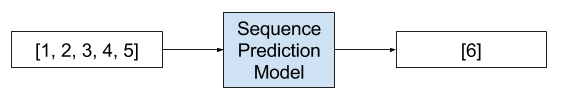
\includegraphics[width=0.7\textwidth]{figures/Example-of-a-Sequence-Prediction-Problem.png}
	\caption{Example of simple sequence prediction}
	\label{fig:exampleSimpleSequencePrediction}
\end{figure}

There are some example of sequence prediction problems, including:


\begin{enumerate}
	\item \textbf{Stock Market Prediction}\cite{Pagolu2016,Liu2018}. Given sequence of stock value as input, predict the expected next stock value. 
	
	\item \textbf{Product Recommendation}\cite{Wang2018,Cao2019}. Given sequence of recent purchased goods of a customer, predict the thing that the customer might "add to cart" next, and then make recommendation. 
	
	\item \textbf{Weather Forecasting}\cite{Quan2000,Wang2017}. Given sequence of weather observation over a period of time, predict the expected weather in next point of time.
	
\end{enumerate}

% Related to water body from satellite images, figure out why it related and its expansion: periodical information

One of important fields of weather forecasting is Nowcasting Precipitation\cite{Sun2013}. The goal of this task is about giving precise prediction of rainfall intensity in a region, over a short period of time. Recent advances in deep learning, Recurrent Neural Networks (RNNs), especially Long Short-Term Memories (LSTMs) models\cite{Graves2013GeneratingSW,Hochreiter1997,Cho2014,Donahue2017} provides good results on this kind of problem. In this chapter, we would like to predict the next water body shape (related to its area), from its time-series data. The common things between nowcasting precipitation and this problem is they both have spatial, spectral and temporal information inside data. We would like to apply model containing Conv-LSTM-2D layer\cite{Shi2015ConvolutionalLN}, to solve our proposed problem. Conv-LSTM-2D layer is recently used in computer vision, especially spatial-temporal problems. In this problem, we would like to extract the spatial feature as well as the correlation in the time. The fully-connected LSTMs can capture the temporal correlation but do not encode the spatial data. That's why they propose a model where the input to state and state to state transitions are convolutional. The model in \cite{Shi2015ConvolutionalLN} show better result on capturing spatial-temporal correlations than other state-of-the-art methods. So in this chapter, we will take this model as reference to provide solution for our problem, for Tri An reservoir.

\section{Dataset} 

In this chapter, Tri An reservoir is chosen for experiments. Because Radar Satellites Images is not affected by cloud cover like optical satellite in \ref{chap-3-recover-water-body}, so we only focus on prediction water body. The synthetic-aperture radar \footnote{https://en.wikipedia.org/wiki/Synthetic-aperture\_radar} monthly imagery provided from Sentinel-1 satellites \footnote{https://sentinel.esa.int/web/sentinel/missions/sentinel-1} are collected from \textit{November 25tr, 2015} to \textit{June 1st, 2019} for training and evaluating. 

Depending on coordinates of Tri An Reservoir, the original image has been cropped to size \textit{2560 px} x \textit{3840 px}, enough to show its water body.

\subsection{Water body segmentation on Sentinel-1 Image}

Sentinel-1 Satellite provides image with 10m spatial resolution. In this chapter, in order to segment out water body, we depend on VH or VV polarizations imagery and apply corresponding threshold:

\begin{equation}
\centering
VH \leq -21
\end{equation} 

\begin{equation}
\centering
VV \leq -17
\end{equation} 

Because in our cropped image that only contains Tri An Reservoir as the largest water body, so we only need to find out the most largest one, using Bread-First Search algorithm\footnote{https://en.wikipedia.org/wiki/Breadth-first\_search}. With this object, we easily to figure out the boundaries, with help of function \textit{find\_boundaries}, from Python library \textit{Scikit-Image}\footnote{https://scikit-image.org/}.

\pagebreak
\section{Model}

The model has been implemented by Keras. Its structure is shown below:

\begin{figure}[h!]
	\centering
	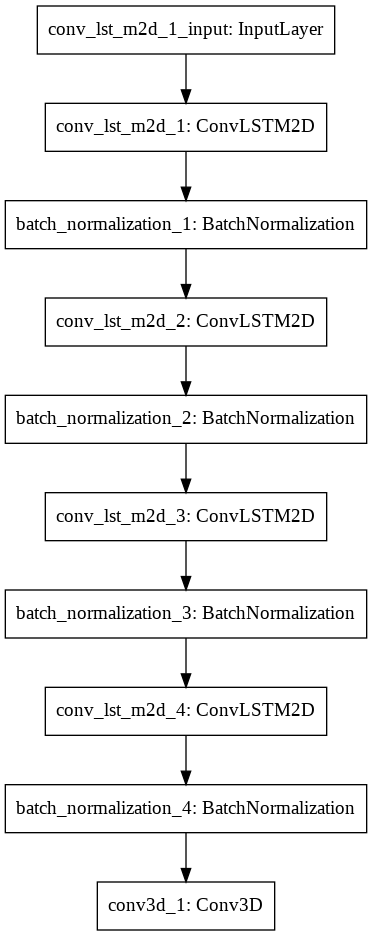
\includegraphics[width=0.4\textwidth]{figures/time_model.png}
	\caption{Prediction mode, based on Conv-LSTM-2D}
	\label{fig:timeModel}
\end{figure}

Model summary detail:

\begin{verbatim}
_________________________________________________________________
Layer (type)                 Output Shape               Param #   
=================================================================
conv_lst_m2d_1 (ConvLSTM2D)  (None, None, 128, 128, 64) 815616    
_________________________________________________________________
batch_normalization_1 (Batch (None, None, 128, 128, 64) 256       
_________________________________________________________________
conv_lst_m2d_2 (ConvLSTM2D)  (None, None, 128, 128, 32) 602240    
_________________________________________________________________
batch_normalization_2 (Batch (None, None, 128, 128, 32) 128       
_________________________________________________________________
conv_lst_m2d_3 (ConvLSTM2D)  (None, None, 128, 128, 32) 401536    
_________________________________________________________________
batch_normalization_3 (Batch (None, None, 128, 128, 32) 128       
_________________________________________________________________
conv_lst_m2d_4 (ConvLSTM2D)  (None, None, 128, 128, 32) 401536    
_________________________________________________________________
batch_normalization_4 (Batch (None, None, 128, 128, 32) 128       
_________________________________________________________________
conv3d_1 (Conv3D)            (None, None, 128, 128, 1)  33        
=================================================================
Total params: 2,221,601
Trainable params: 2,221,281
Non-trainable params: 320
_________________________________________________________________
\end{verbatim}

Specification:

\begin{itemize}
	\item \textit{Input and Output} Because we only focus on predicting water body, so after extracting water body from original image and finding out its boundaries, we randomize on boundaries 50 tiles with size of 128 x 128. There is 12 consecutive images, corresponding to 12 month in year. The output is a image of next month, which is same month of 1st image in input sequence but next year. 
	
	\item \textit{Conv3D} This type of layer helps to catch spatial and temporal invariances in the same manner as \textit{Conv2D} in an imagery case. This make the curse of dimensionality much less harmful. Because at the end of model, we need to have a prediction, so it's no longer to keep temporal information after this layer.
	
	\item \textit{Batch Normalization} Batch normalization reduces the amount by what the hidden unit values shift around (covariance shift). Morever, this layer allows each layer of a network to learn by itself a little bit more independently of other layers.
	
	\item \textit{Activation} The activation for Conv-LSTM-2D is $tanh$ function, for Conv3D is $sigmoid$ function.
	
	\item \textit{Dropout and Recurrent Dropout} In Recurrent Neural Networks, we have two definition about \textbf{Dropout} and \textbf{Recurrent Dropout}. \textbf{Dropout} describes fraction of the units to drop for the linear transformation of the inputs, while \textbf{Recurrent Dropout} show fraction of the units to drop for the linear transformation of the recurrent state (more detail at \cite{Gal2015}). In this model, with each Conv-LSTM-2D layer's configuration, $dropout$ is set at $0.4$, and and $recurrent\_dropout$ is $0.3$.
	
	\item \textit{Model compilation parameters} Like model compilation in \ref{chap-3-recover-water-body}, the loss function is still $mean\_square\_error$, optimizer is $adam$ and evaluation metric is $PSNR$(\ref{psnr_eq}). 
	
\end{itemize}

\section{Experiments}

\subsection{Prediction water body area}

% Show demo 12 input in 1 line


The time-series data in one year (one file per month) has been divided into tile of \textit{128 px } x \textit{128 px}. All tiles belong to wate body are predicted but only area and boundaries of water body are evaluated. Figure \ref{fig:inputTs} show the sample input from June 2018 to May 2019, and the groundtruth of the next point of time, which is retrieved in June 2019, is shown at Figure \ref{fig:outputTs}.

\begin{figure}[h!]
	\centering
	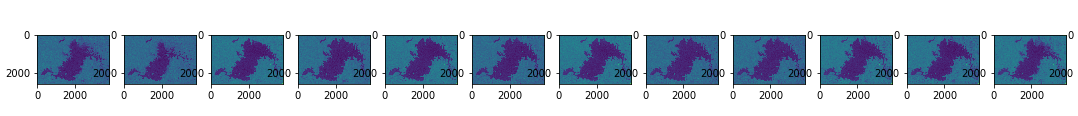
\includegraphics[width=1\textwidth]{figures/input_ts.png}
	\caption{Sample input for prediction model, in term of temporal (from left to right: June 2018 to May 2019)}
	\label{fig:inputTs}
\end{figure}

\begin{figure}[h!]
	\centering
	\includegraphics[width=0.5\textwidth]{figures/output_ts.png}
	\caption{Sample output: Groundtruth of water body in next time of sequence, June 2019.}
	\label{fig:outputTs}
\end{figure}

The prediction result of model, from Feb 2019 to June 2019 is shown in table \ref{table:predictValue}.

% Show table, contains result

\begin{table}[h!]
	\centering
	\begin{tabularx}{\textwidth}{|c|Y|Y|Y|Y|}
		\hline
		\textbf{Month} & \textbf{Groundtruth Area ($km^2$)} & \textbf{Predicted Area ($km^2$)} & \textbf{True Prediction Ratio (\%)} & \textbf{False Prediction Ratio (\%)}\\ \hline
		2              & 282.5946                                          & 287.7469                                        & 98.32 & 3.44                         \\ \hline
		3              & 296.5101                                          & 301.0503                                        & 97.02 & 
		4.44                          \\ \hline
		4              & 301.2402                                          & 276.8264                                        & 87.60 & 4.68                         \\ \hline
		5              & 273.7712                                          & 273.0462                                        & 96.39 & 3.35                          \\ \hline
		6              & 243.2829                                          & 217.7548                                        & 86.40 & 3.47                         \\ \hline
	\end{tabularx}
	\caption{Area prediction result and ratio}
	\label{table:predictValue}
\end{table}

% Plot predicted result, with groundtruth value

\begin{figure}[h!]
	\centering
	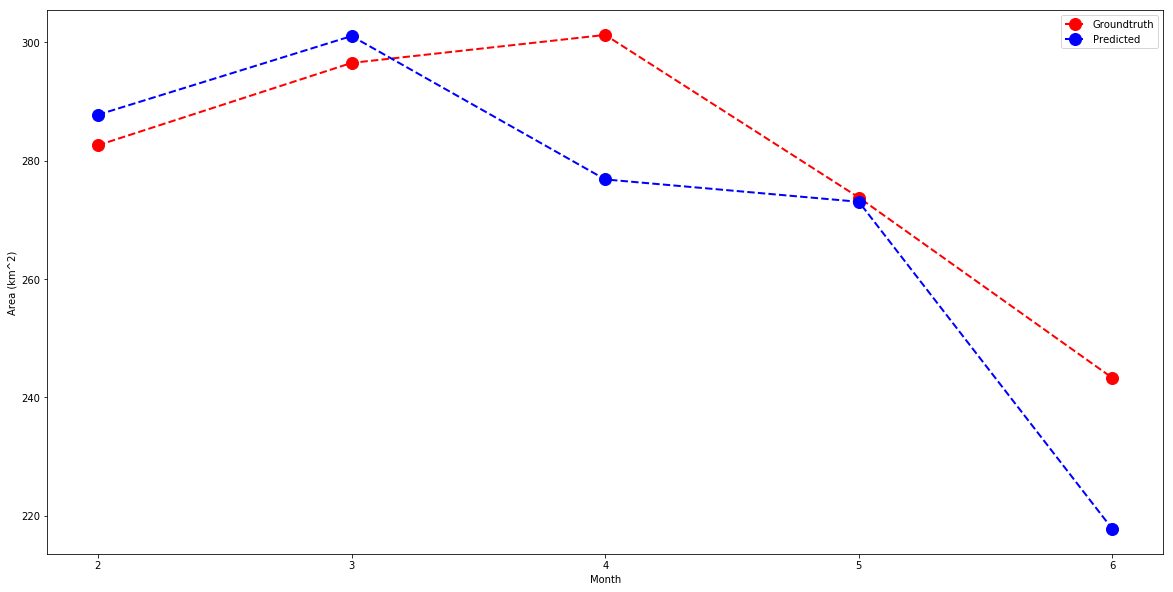
\includegraphics[width=1\textwidth]{figures/comparePredict.png}
	\caption{Area comparison between groundtruth and prediction.}
	\label{fig:comparePredict}
\end{figure}

Below are prediction and groundtruth for Tri An Reservoir water body, from February to June 2019, while the yellow line shows boundaries of predicted water body:

% Show 2-6/19 prediction, with result and boundaries.
\begin{figure}[h!]
	\centering
	\includegraphics[width=0.9\textwidth]{figures/20190202T110307.png}
	\caption{Prediction, Feb 2019}
\end{figure}

\begin{figure}[h!]
	\centering
	\includegraphics[width=0.9\textwidth]{figures/20190309T223707.png}
	\caption{Prediction, March 2019}
\end{figure}

\begin{figure}[h!]
	\centering
	\includegraphics[width=0.9\textwidth]{figures/20190402T223708.png}
	\caption{Prediction, April 2019}
\end{figure}

\begin{figure}[h!]
	\centering
	\includegraphics[width=0.9\textwidth]{figures/20190508T223709.png}
	\caption{Prediction, May 2019}
\end{figure}

\begin{figure}[h!]
	\centering
	\includegraphics[width=0.9\textwidth]{figures/20190601T223710.png}
	\caption{Prediction, June 2019}
\end{figure}


\subsection{Example with anomaly detection}
\label{section:anomalyDetection}

One usage of sequence prediction output is about anomaly detection. This problem is usually formulated as finding outlier data points, relative to some standard or usual signal. In this chapter, the data points show water body area of Tri An Reservoir. The below chart show observations of Tri An reservoir area in 3 years, from 2016-2018.

\begin{figure}[h!]
	\centering
	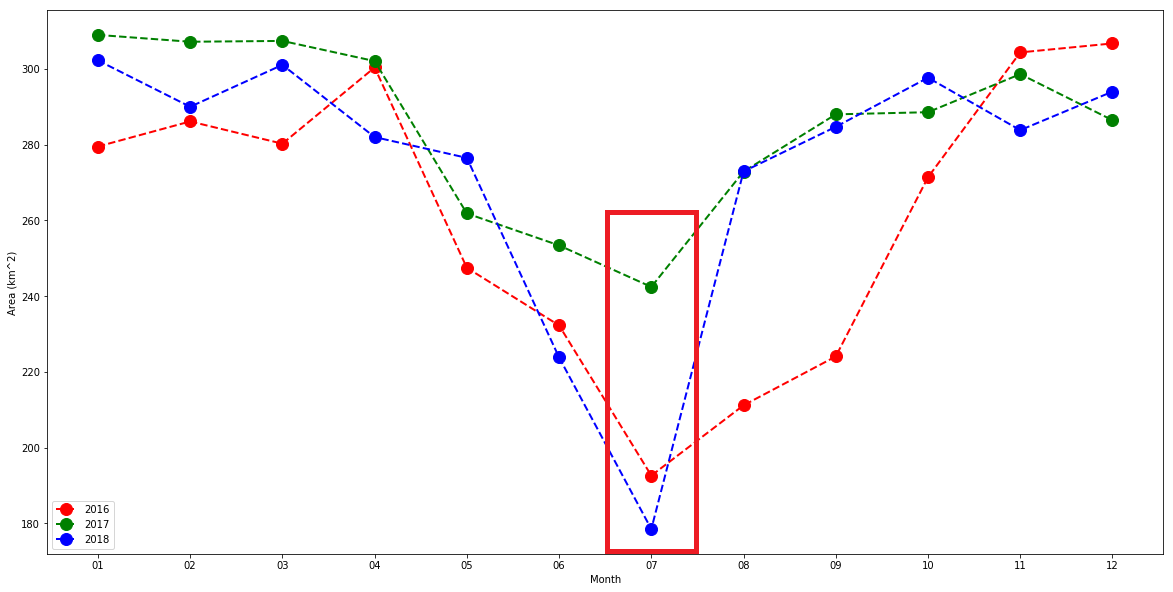
\includegraphics[width=0.9\textwidth]{figures/observations.png}
	\caption{Observations of Tri An reservoir from Sentinel-1 Satellite, in term of water body area. Notice that, on July 2017, the water body area is seemed to be different from year 2016 and 2018}
	\label{fig:observation}
\end{figure}

Following observations, the groundtruth area of water body in 2016, 2017 and 2018 are $189.6926 km^2$, $242.4104 km^2$ and $178.4857 km^2$ respectively. While using our model, the prediction is approximately $189.6926 km^2$. See more about visualization at Fig. \ref{fig:anomalyVis} and graph for comparison at Fig. \ref{fig:anomalyComp}

\begin{figure}[h!]
	\centering
	\includegraphics[width=0.9\textwidth]{figures/20170706T110259.png}
	\caption{Prediction for July 2017, using 12 previous data points (from July 2016 to Jun 2017)}
	\label{fig:anomalyVis}
\end{figure}


\begin{figure}[h!]
	\centering
	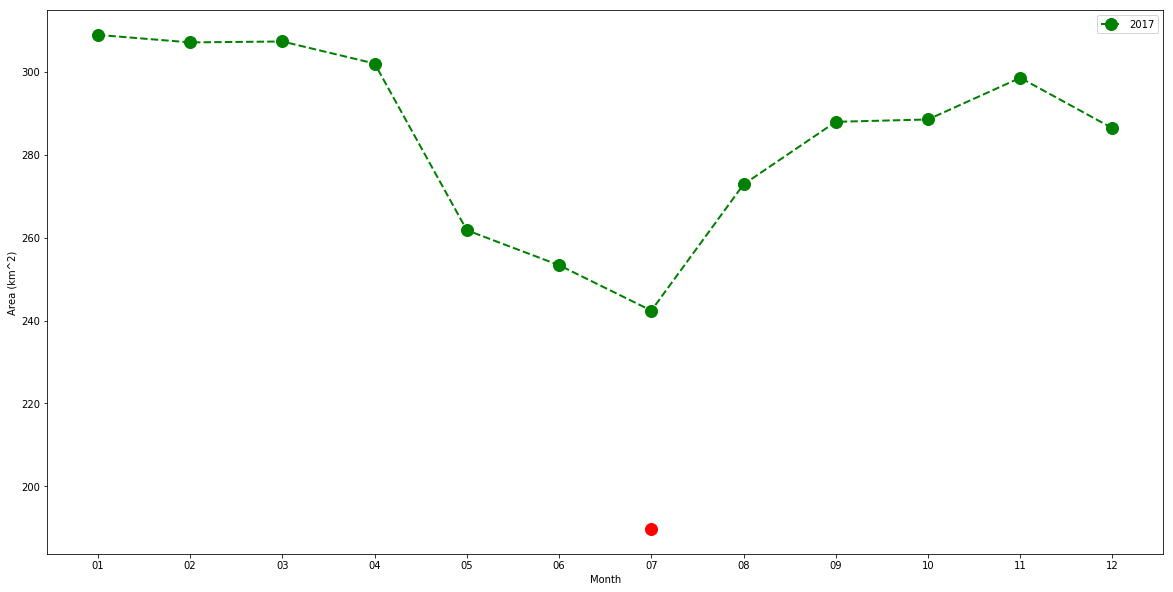
\includegraphics[width=0.9\textwidth]{figures/anomaly.png}
	\caption{Prediction (the red point) and groundtruth (the green line) on July 2017}
	\label{fig:anomalyComp}
\end{figure}

\section{Conclusions}

In this chapter, we have a very good result on applying deep learning to prediction problem on Tri An Reservoir. This potential result may help us a lot when dealing with sequence prediction problem, especially complicated situation, such as spatial-temporal sequence forecasting problem, using proposed extension of LSTM - Conv-LSTM-2D. Beside that, with accepted prediction, the output of this problem may be used on other sequence problems, such as anomaly detection that we've taken example in \ref{section:anomalyDetection}. For future work, when enough data for training and testing, an end-to-end real-time forecasting water body observer system might be proposed, with two main parts: Prediction part and classification for anomalies part. 